\documentclass[a4paper,10pt,border=8pt]{report}
% \usepackage[a4paper,top=3cm,bottom=3.5cm,left=3cm,right=3cm,bindingoffset=5mm]{geometry}

\usepackage{graphicx}
\usepackage{float}
\usepackage{amsmath}       
\usepackage{scalefnt}
\usepackage[dvipsnames]{xcolor}
%% TIKZ
\usepackage{tikz}
\usepackage{pgfplots}
\pgfplotsset{compat=newest}
\usepgfplotslibrary{external} 
\usetikzlibrary{external} 
\tikzexternalize[prefix=tikz/]
\usetikzlibrary{mindmap}
\usetikzlibrary{decorations.pathmorphing,decorations.text,decorations.pathreplacing}
\usetikzlibrary{patterns}
\usetikzlibrary{shapes,shapes.multipart,arrows,fit,calc,positioning,intersections,through}
\usetikzlibrary{backgrounds,fadings}
\newcommand{\pin}[4]{
	    node[pos=#1,coordinate,pin={[pin distance=#4,pin edge={line to,-,shorten <=0ex}]#2,left,inner sep=0pt:{#3}}] {}
}
\newcommand{\pinc}[5]{
	    node[pos=#1,coordinate,pin={[pin distance=#4,pin edge={color = #5,line to,-,shorten <=0ex}]#2,left,inner sep=0pt:{\textcolor{#5} #3}}] {}
}
\newcommand{\did}[1]{\caption{\emph{\small{#1}}}}
\tikzset{
  text deco/.style={
    postaction={decorate, decoration={text along path, #1}}}}
 
\newcommand*{\boxcolor}{orange}
\makeatletter
\renewcommand{\boxed}[2]{\textcolor{#2}{%
% \def\larg {width(" $\omega$ ")+2 pt}
\tikz[
baseline={([yshift=-1ex]current bounding box.center)}
] \node [rectangle,rounded corners,draw, fill=#2!20,inner sep = 1.5pt, outer sep = 0.pt] {\normalcolor\m@th$#1$};}}
 \makeatother
 
\makeatletter
\newcommand{\imagebox}[3]{
\textcolor{#2}{%
\tikz[baseline={([yshift=-1ex]current bounding box.center)}] \node [rectangle, minimum width=1ex,rounded corners,draw, fill=#2!10, inner sep = 1.5pt,outer sep=0.pt] (#3) {#1};
}}
 \makeatother  
 
 % % % first_palette
\definecolor{bcolor1}{HTML}{703517}
\definecolor{bcolor2}{HTML}{5D432A}
\definecolor{bcolor3}{HTML}{7D7B64}
\definecolor{bcolor4}{HTML}{7B886E}
\definecolor{bcolor5}{HTML}{B95613}
\definecolor{bcolor6}{HTML}{B95613}
\definecolor{bcolor7}{HTML}{756555}
\definecolor{bcolor8}{HTML}{6F9065}
\definecolor{bcolor9}{HTML}{7ACEF3}%blockblue
\definecolor{bcolor10}{HTML}{FF8A00}%blockorange
\definecolor{bcolor11}{HTML}{CCCCCC}
\definecolor{bcolor12}{HTML}{8C8C8C}
\definecolor{bcolor13}{HTML}{737373} 
\definecolor{bcolor14}{HTML}{4D4D4D} 
 \definecolor{burntsienna}{rgb}{0.91, 0.45, 0.32}
 \definecolor{candyapplered}{rgb}{1.0, 0.03, 0.0}
 
%%%%%%%%%%%%%%%%%%%%%%%%%%%%%%%%%%%%%%%%%%%%%%%%%%%%%%%%%%%%%%%%%%%%%%%%%%%%%%%%%%%%%%%%%%%%%%%%%%
\begin{document}
 \tikzsetnextfilename{flow_chart}
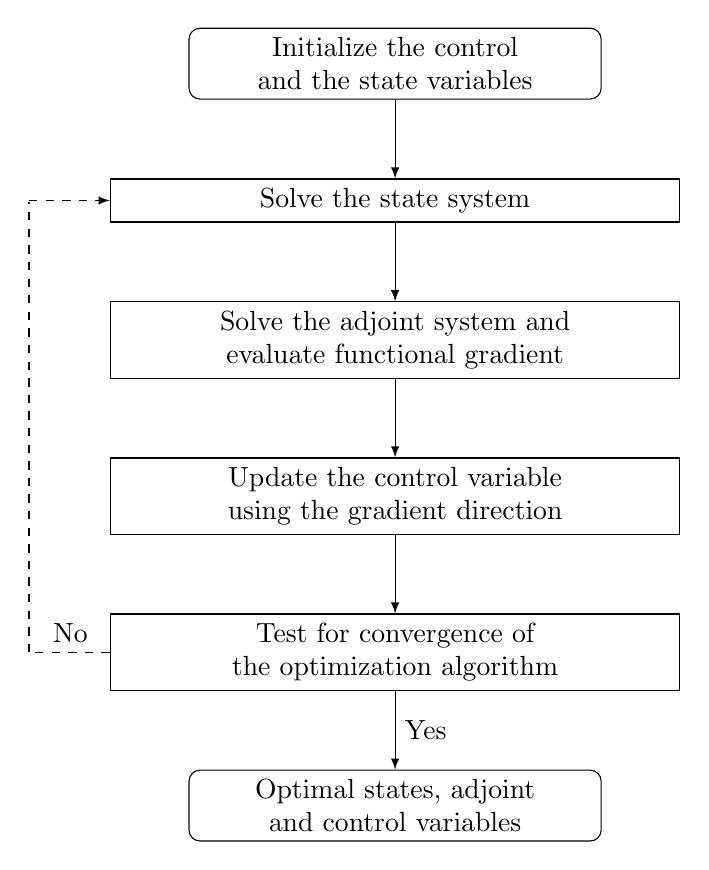
\begin{tikzpicture}[>=latex]
%     every node/.style = {thin, shape=rectangle, 
%    rounded corners,
%     draw, 
%     align=center},
%    ]    
\node[thin, shape=rectangle,rounded corners,draw,align=center, text width = 5cm ](point1)  {Initialize the control and the state variables};
\node[thin, shape=rectangle,draw,align=center, text width = 7cm, below=of point1 ](point2) {Solve the state system};
\node[thin, shape=rectangle,draw,align=center, text width = 7cm, below=of point2 ](point3) {Solve the adjoint system and evaluate functional gradient};
\node[thin, shape=rectangle,draw,align=center, text width = 7cm, below=of point3 ](point4) {Update the control variable using the gradient direction };
\node[thin, shape=rectangle,draw,align=center, text width = 7cm, below=of point4 ](point5) {Test for convergence of the optimization algorithm};
\node[thin, shape=rectangle,rounded corners,draw,align=center, text width = 5cm, below=of point5](point6) {Optimal states, adjoint and control variables};
\node[left=of point5.west, inner sep=0pt](point6) {};
\node[left=of point2.west, inner sep=0pt ](point8) {};
\draw[thin,dashed] (point5) -- node[near start,above, midway] {No} (point6);
\draw[thin,dashed] (point6) -| (point8);
\draw[thin, ->, dashed] (point8) |- (point2);
\draw[thin, ->] (point1) -- (point2);
\draw[thin, ->] (point2) -- (point3);
\draw[thin, ->] (point3) -- (point4);
\draw[thin, ->] (point4) -- (point5);
% \draw[thin, ->] (point5) -- (point6);
%\draw[thin,->] (0,0) -- (4.5,0);
%\draw[thin] (point9) -| node[near start,above] {} (point2);
% \draw[thin,->] (point7) -- (point9) node[] {};
\node[below=of point5.south ](point7) {};
\draw[thin,->] (point5) -- (point7) node[midway,right] {Yes};
% \draw[->,>=latex] (point0.east) to[out=0,in=180]  (point1.west);
% \node[right=of point1.east, xshift=-0.35cm, fill=corn, text width =2.2cm ](point11) {Calcolo $\mathcal{J}^0$};
% \draw[->,>=latex] (point1.east) to[out=0,in=180]  (point11.west);
% \node[below=of point1.south, yshift=0.8cm, fill=coral,text width = 3cm ](point2) {\textbf{Risoluzione equazioni aggiunte}\\$(\vect{u}_a^i,p_a^i,k_a^i,\omega_a^i,\nu_a^i)$};  
% \node[below=of point0.south, left=of point2.west, fill=coral, text width=2cm ](for) {Ciclo esterno $i=1,\dots$};     
% \node[below=of point2.south,yshift=0.8cm,xshift=0cm, fill=columbiablue,text width = 3cm ](agg) {$\vect{f}^i=\vect{f}^{i-1}+\rho^{i,j}\frac{\vect{u}_a^i}{\lambda}$};     
% \node[below=of for.south, left=of agg.west, fill=columbiablue, text width=1.8cm ](for1) {\footnotesize Ciclo interno $j=0,\dots$};   
% \node[below=of agg.south,yshift=1cm,xshift=0cm, fill=columbiablue,text width = 3.2cm ](RANS) {\textbf{Risoluzione sistema RANS} $k$-$\omega$\\$(\vect{u}^{i,j},p^{i,j},k^{i,j},\omega^{i,j},\nu_t^{i,j})$};
% \node[below=of RANS.south, xshift=0cm,yshift=1cm,fill=columbiablue, text width =2.cm](Ji) {Calcolo $\mathcal{J}^{i,j}$};
% \node[right=of Ji.east, xshift=1.8cm,yshift=0cm](A) {};
% \node[right=of Ji.east, xshift=-1cm,yshift=-0.4cm](B) {se\\ $\mathcal{J}^{i,j}-\mathcal{J}^{i,j-1}>0$};
% \node[right=of Ji.east, xshift=1.4cm, fill=columbiablue, text width=2cm ](for2) {$j=j+1$ \\$\rho^{i,j+1}=0.7\rho^{i,j}$};   
% \draw[->,>=latex] (Ji.east) to[]  (for2.west);
% \node[left=of Ji.west, xshift=1cm,yshift=-0.4cm](C) {se\\ $\mathcal{J}^{i,j}-\mathcal{J}^{i,j-1}<0$};  
% \node[left=of Ji.west, xshift=-1.2cm,fill=coral, text width=1.5cm ](for3) {$i=i+1$};  
% \draw[->,>=latex] (Ji.west) to[]  (for3.east);
% \node[below=of Ji.south, yshift=-0.5cm, fill=etonblue](D) {$\vect{f}$ ottimo}; 
% \draw[->,>=latex] (Ji.south) to[]  (D.north);
% \node[right=of D.east,xshift=-1cm](E) {se $\dfrac{||\mathcal{J}^{i,j}-\mathcal{J}^{i,j-1}||}{\mathcal{J}^{i,j-1}}<toll$}; 
\end{tikzpicture}
\end{document}
% pdflatex --shell-escape figure.tex
